\chapter{Реализация прототипа плагина} \label{ch3}

% не рекомендуется использовать отдельную section <<введение>> после лета 2020 года
%\section{Введение. Сложносоставное название первого параграфа первой главы для~демонстрации переноса слов в содержании} \label{ch1:intro}
В 3 главе будут рассмотрены и описаны основные классы, которые были разработаны в соотвествии с диаграммой классов из приложения 1, а также полученные результаты.

\section{Описание разработанных классов} \label{ch3:sec1}

В процессе написания кода плагины были запрограммированы следующие классы:

\begin{itemize}
	\item BuildConfigurationStatisticsAction - базовый класс приложения, который реализует интерфейс действия, через этот класс происходит взаимодействие с Jelly, а также вызов всех остальных методов бизнес-логики плагина, и определены поля для работы со сборками, все методы для получения информации о крнкретной метрике сборки помечены аннотацией @JavaScript для того, чтобы можно было их вызывать через JS в Jelly, также во всех этих методах тип возвращаемого объекта приведен к JSON, который и передается в DOM страницы плагина при взаимодействии с элементами пользовательского интерфейса;
	\item DateTimeHandler - статический класс, созданный для взаимодействия с датами и их обработки при создании структур данных, которые также создаются в рамках этого класса, формирования структуры данных зависит от метрики и от периода за который нужно получить информацию;
	\item IntervalDate - перечисляемый тип для удобства работы с датами-периодами;
	\item TimeInQueueFetcher - класс отвечающий за расчет времени, которая сборка провела в очереди перед тем как отправилась на выполнение;
	\item BuildLogic - базовый класс бизнес-логики, от которого наследуются все остальные более специфичные классы по каждой метрике, в классе определяются методы фильтрации по периоду и наличию упавших сборок в итоговых результатах;
	\item BuildArtifactSizeLogic - класс для работы с метрикой AS, в нем происходит пересчет параметров в зависимости от периода и настроек подданных на вход, а также высчитывается размер артифакта в Кб;
	\item BuildDurationLogic - класс для работы с метрикой BD, в нем происходит пересчет параметров в зависимости от периода и настроек подданных на вход, а также высчитывается продолжительность сборки в секундах;
	\item BuildSuccessRateLogic - класс для работы с метрикой SR, в нем происходит пересчет параметров в зависимости от периода, а также высчитывается процент успешности выполненных сборок за заданный промежуток времени;
	\item BuildTestCountLogic - класс для работы с метрикой TS, в нем происходит пересчет параметров в зависимости от периода и настроек подданных на вход, а также высчитывается количество выполненных тестов во время работы сборок за определенный период;
	\item BuildTimeQueueLogic - класс для работы с метрикой BQ, в нем происходит пересчет параметров в зависимости от периода и настроек подданных на вход, а также высчитывается время ожидание сборки в очереди в милисекундах.
\end{itemize}

В JS определяются функции событий для выбора элемента из выпадающего списка и взаиможействия с флажками. Для каждой метрики используется своя функции, внутри определяются настройки данных и отображения для визуализации отдельной метрики в виде определенного графика/диаграммы, вызывается метод для сортировки агрегированных по датам значений метрик в структуре JSON, а также формируются метки-подписи для каждого типа периода.

В jelly файле с помощью html формируется структура документа, а также выполняется привязка Java объектов к объектам JS. Определяются обработчики событий, который при взаимодействии с пользователем вызывают определенный запрос-метод AJAX.

\section{Результаты разработки плагина} \label{ch3:sec2}

При разработке плагина надо было учитывать, что требуется отображать все графики на одной странице задания друг под другом, поскольку при выборе одно периода, например, месяца, будет получена сводная информация по каждой сборке или нескольких сборок запущенных в один день. Графики отображаются посредством переходна на соотвествующую ссылку, оставляя при этом пользователя в том же задании (странице с результатами последних сборок).

В интерфейсе у каждого графика были реализованы те дополнительные функции отображения, которые могут быть применины к визуализируемой метрике: отобразить статистику по упавшим сборкам/тестам, усреднить метрику.

Интерфейс страницы плагина с графиками в системе Jenkins на странице задания показан на рисунке 3.1.


\begin{figure}[ht!] 
	\center
	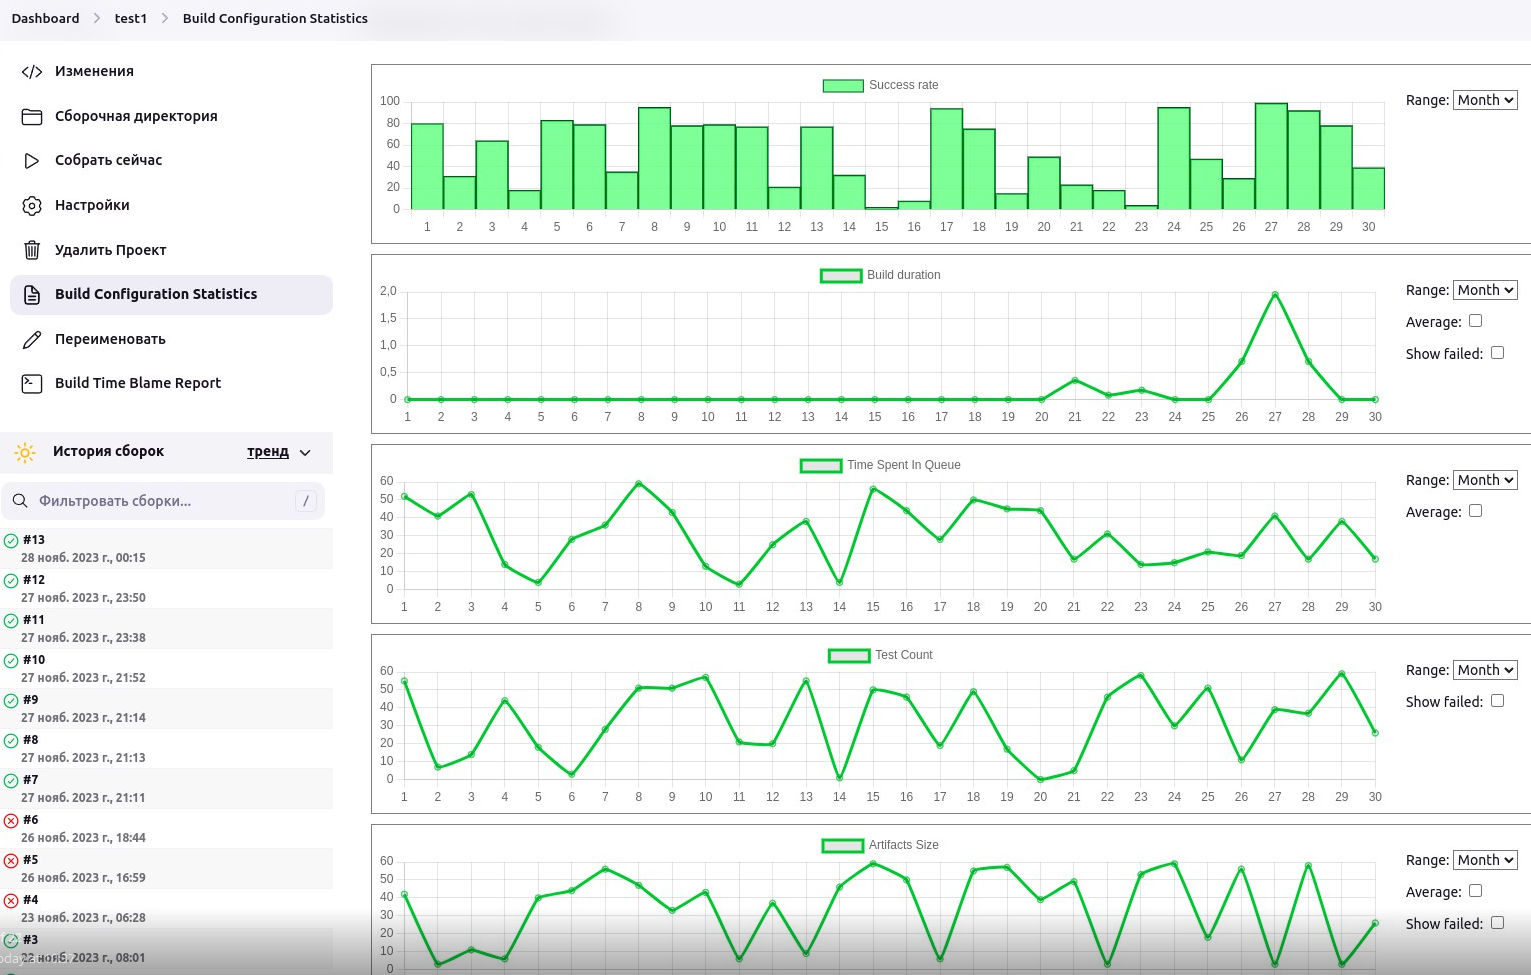
\includegraphics [scale=0.47] {my_folder/images//ui}
	\caption{Интерфейс плагина Jenkins} 
	\label{fig:ArchitectureJenkins}  
\end{figure}

Интерфейс страницы плагина с графиками в системе Jenkins на странице задания при выборе всех включенных настроек, а также с выбранным периодом неделя показан на рисунке 3.2.

\begin{figure}[ht!] 
	\center
	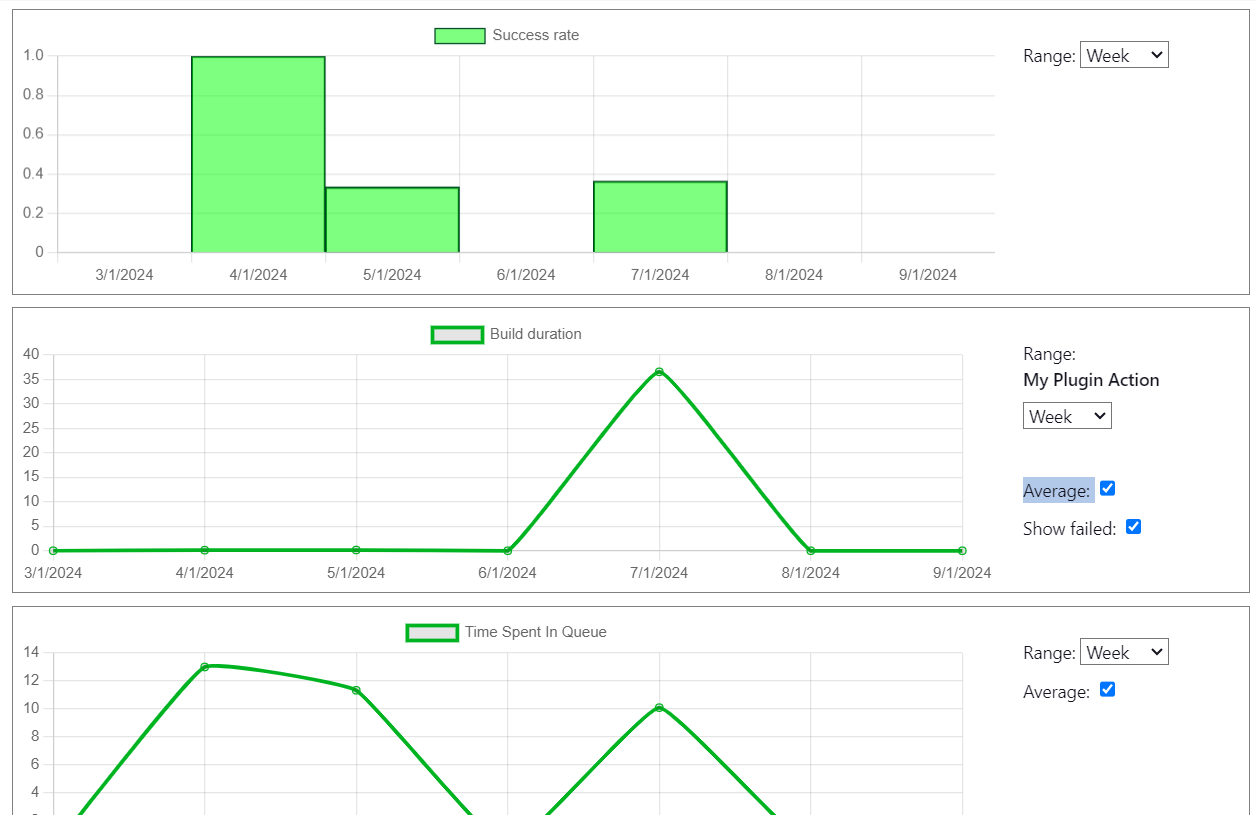
\includegraphics [scale=0.47] {my_folder/images//ui4}
	\caption{Интерфейс графиков с включенным настройками и периодом неделей} 
	\label{fig:ArchitectureJenkins}  
\end{figure}

Основное взаимодействие с графиками будет производить через меню, которое есть напротив каждого графика со своими параметрами, отображенном на рисунке 3.3:

\begin{figure}[ht!] 
	\center
	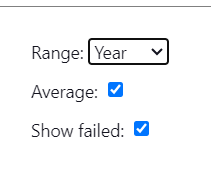
\includegraphics [scale=0.47] {my_folder/images//ui2}
	\caption{Интерфейс элементов управления} 
	\label{fig:ArchitectureJenkins}  
\end{figure}

При взаимодействии с раскрывающимся списком должен вызываться Java метод, который пересчитает и отфильтрует необходимые сборки Jenkins и динамически отобразит результаты по выбранными периоду, также динамически должна производить обработка метрик сборок, при выборе основной метрики ни как суммы всех значений, а как среднего, а также включение в графики данных об упавших сборках, при выборе соотвествующих чекбоксов.

Интерфейс изменения навигационной панели отображен на рисунке 3.4. В данном случае видно что изменения видны при открытии конфигурации конкретной сборки, т.е. не надо будет переключаться между окном плагина и сборкой для визуализации метрик, при открытии данного пункта меню, также происходит изменения URL, с которым в дальнейшем и происходит взаимодействие.

\begin{figure}[ht!] 
	\center
	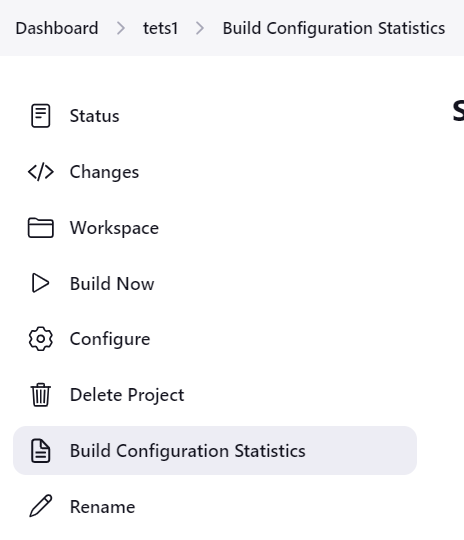
\includegraphics [scale=0.47] {my_folder/images//ui3}
	\caption{Интерфейс элементов управления} 
	\label{fig:ArchitectureJenkins}  
\end{figure}


Код плагина представлен в приложении 4.
 
\section{Выводы} \label{ch3:sec3}

В главе 3 была проведена реализация плагина, а также описаны классы, разработанные при написании плагина и файлы, которые участвуют во взаимодействии с этими классами и отображаемым интерфейсом пользователя. Также были приведены результаты разработкы, приведены скриншоты интерфейсов, а также описаны добавленные на страницу Jenkins элементы, после установки плагина.





%
%

%
%
%\begin{table} [htbp]% Пример оформления таблицы
%	\centering\small
%	\caption{Представление данных для сквозного примера по ВКР \cite{Peskov2004}}%
%	\label{tab:ToyCompare}		
%		\begin{tabular}{|l|l|l|l|l|l|}
%			\hline
%			$G$&$m_1$&$m_2$&$m_3$&$m_4$&$K$\\
%			\hline
%			$g_1$&0&1&1&0&1\\ \hline
%			$g_2$&1&2&0&1&1\\ \hline
%			$g_3$&0&1&0&1&1\\ \hline
%			$g_4$&1&2&1&0&2\\ \hline
%			$g_5$&1&1&0&1&2\\ \hline
%			$g_6$&1&1&1&2&2\\ \hline		
%		\end{tabular}	
%	\normalsize% возвращаем шрифт к нормальному
%\end{table}


% \firef{} от figure reference
% \taref{} от table reference
% \eqref{} от equation reference




